\documentclass{article}


% if you need to pass options to natbib, use, e.g.:
%     \PassOptionsToPackage{numbers, compress}{natbib}
% before loading neurips_2025


% ready for submission
%\usepackage{neurips_2025}


% to compile a preprint version, e.g., for submission to arXiv, add add the
% [preprint] option:
\usepackage[preprint]{neurips_2025}


% to compile a camera-ready version, add the [final] option, e.g.:
%     \usepackage[final]{neurips_2025}


% to avoid loading the natbib package, add option nonatbib:
%    \usepackage[nonatbib]{neurips_2025}


\usepackage[utf8]{inputenc} % allow utf-8 input
\usepackage[T1]{fontenc}    % use 8-bit T1 fonts
\usepackage{hyperref}       % hyperlinks
\usepackage{url}            % simple URL typesetting
\usepackage{booktabs}       % professional-quality tables
\usepackage{amsfonts}       % blackboard math symbols
\usepackage{nicefrac}       % compact symbols for 1/2, etc.
\usepackage{microtype}      % microtypography
\usepackage{xcolor}         % colors

\usepackage{bm}
\usepackage{enumerate}
\usepackage{amsmath}
\usepackage{amssymb}
\usepackage{amsthm}
\usepackage{mathtools}
\usepackage{algorithm}
\usepackage{algorithmic}

\theoremstyle{plain}
\newtheorem{theorem}{Theorem}
\newtheorem{proposition}{Proposition}
\newtheorem{lemma}{Lemma}
\newtheorem{corollary}{Corollary}
\theoremstyle{definition}
\newtheorem{definition}{Definition}
\newtheorem{assumption}{Assumption}
\newtheorem{example}{Example}
\theoremstyle{remark}
\newtheorem{remark}{Remark}

\renewcommand{\algorithmicrequire}{\textbf{Input:}}
\renewcommand{\algorithmicensure}{\textbf{Output:}}

\title{BNPO: Beta Normalization Policy Optimization}


% The \author macro works with any number of authors. There are two commands
% used to separate the names and addresses of multiple authors: \And and \AND.
%
% Using \And between authors leaves it to LaTeX to determine where to break the
% lines. Using \AND forces a line break at that point. So, if LaTeX puts 3 of 4
% authors names on the first line, and the last on the second line, try using
% \AND instead of \And before the third author name.


\author{%
  Changyi Xiao\textsuperscript{\rm 1}, Mengdi Zhang\textsuperscript{\rm 2}, Yixin Cao\textsuperscript{\rm 1}\thanks{Corresponding author.} \\
  \textsuperscript{\rm 1}School of Computer Science, Fudan University\\
    \textsuperscript{\rm 2}Meituan Group\\
  \texttt{\{changyi\_xiao, yxcao\}@fudan.edu.cn}\\
  % examples of more authors
  % \And
  % Coauthor \\
  % Affiliation \\
  % Address \\
  % \texttt{email} \\
  % \AND
  % Coauthor \\
  % Affiliation \\
  % Address \\
  % \texttt{email} \\
  % \And
  % Coauthor \\
  % Affiliation \\
  % Address \\
  % \texttt{email} \\
  % \And
  % Coauthor \\
  % Affiliation \\
  % Address \\
  % \texttt{email} \\
}



\begin{document}


\maketitle


\begin{abstract}
Recent studies, including DeepSeek-R1 and Kimi-k1.5, have demonstrated that reinforcement learning with rule-based, binary-valued reward functions can significantly enhance the reasoning capabilities of large language models. These models primarily utilize REINFORCE-based policy optimization techniques, such as REINFORCE with baseline and group relative policy optimization (GRPO). However, a key limitation remains: current policy optimization methods either neglect reward normalization or employ static normalization strategies, which fail to adapt to the dynamic nature of policy updates during training. This may result in unstable gradient estimates and hinder training stability. To address this issue, we propose Beta Normalization Policy Optimization (BNPO), a novel policy optimization method that adaptively normalizes rewards using a Beta distribution with dynamically updated parameters. BNPO aligns the normalization with the changing policy distribution, enabling more precise and lower-variance gradient estimation, which in turn promotes stable training dynamics. We provide theoretical analysis demonstrating BNPO's variance-reducing properties and show that it generalizes both REINFORCE and GRPO under binary-valued reward settings. Furthermore, we introduce an advantage decomposition mechanism to extend BNPO’s applicability to more complex reward systems. Experimental results confirm that BNPO achieves state-of-the-art performance among policy optimization methods on reasoning tasks. The code is available at \url{https://github.com/changyi7231/BNPO}.
\end{abstract}

\section{Introduction}
Kimi-K1.5 \citep{team2025kimi} and DeepSeek-R1 \citep{guo2025deepseek} have demonstrated that reinforcement learning can substantially enhance the reasoning capabilities of large language models. These models leverage reinforcement learning techniques built on rule-based, binary-valued outcome reward functions, and utilize policy optimization techniques such as REINFORCE with baseline \citep{kool2019buy} and group relative policy optimization (GRPO) \citep{shao2024deepseekmath}.


In contrast to proximal policy optimization (PPO) \citep{schulman2017proximal}, which employs a critic network to estimate the baseline for policy gradients, REINFORCE with baseline and GRPO utilize Monte Carlo sampling for baseline estimation, reducing memory and computational overhead. Specifically, REINFORCE with baseline incorporates a state-dependent baseline compared to vanilla REINFORCE to reduce gradient variance, while GRPO further stabilizes training by normalizing rewards, thereby reducing gradient variance in high-variance reward scenarios.

Despite these advances, a fundamental limitation remains: current methods either lack reward normalization entirely or use fixed normalization terms throughout training. This is suboptimal, as the policy model evolves during training, fixed normalization cannot adapt to such dynamics, potentially resulting in inaccurate gradient estimates and unstable learning.

To overcome this limitation, we propose a novel policy optimization method, called Beta Normalization Policy Optimization (BNPO), which dynamically normalizes the reward function using a Beta distribution with its adaptive parameters. By evolving alongside the policy model, this normalization mechanism provides more accurate and lower-variance gradient estimates. Besides, we introduce an advantage decomposition mechanism to enhance BNPO’s ability to handle complex reward systems.

Our approach is motivated by the observation that, under binary-valued reward functions, the reward can be seen as a random variable with Bernoulli distribution, and its expectation naturally can be modeled as a random variable with Beta distribution. As training progresses and the policy evolves, the distribution of expected rewards also shifts. BNPO explicitly accounts for these shifts by adjusting the normalization term accordingly.

We further present a theoretical analysis demonstrating that BNPO can effectively reduce the variance of policy gradient estimates when the Beta distribution parameters are appropriately set. Moreover, we show that BNPO generalizes both REINFORCE and GRPO in the binary-valued reward setting, highlighting its broad applicability and theoretical consistency. Finally, experimental results show that BNPO achieves state-of-the-art performance in policy optimization for reasoning tasks.


\begin{figure}[t]
\begin{center}
\centerline{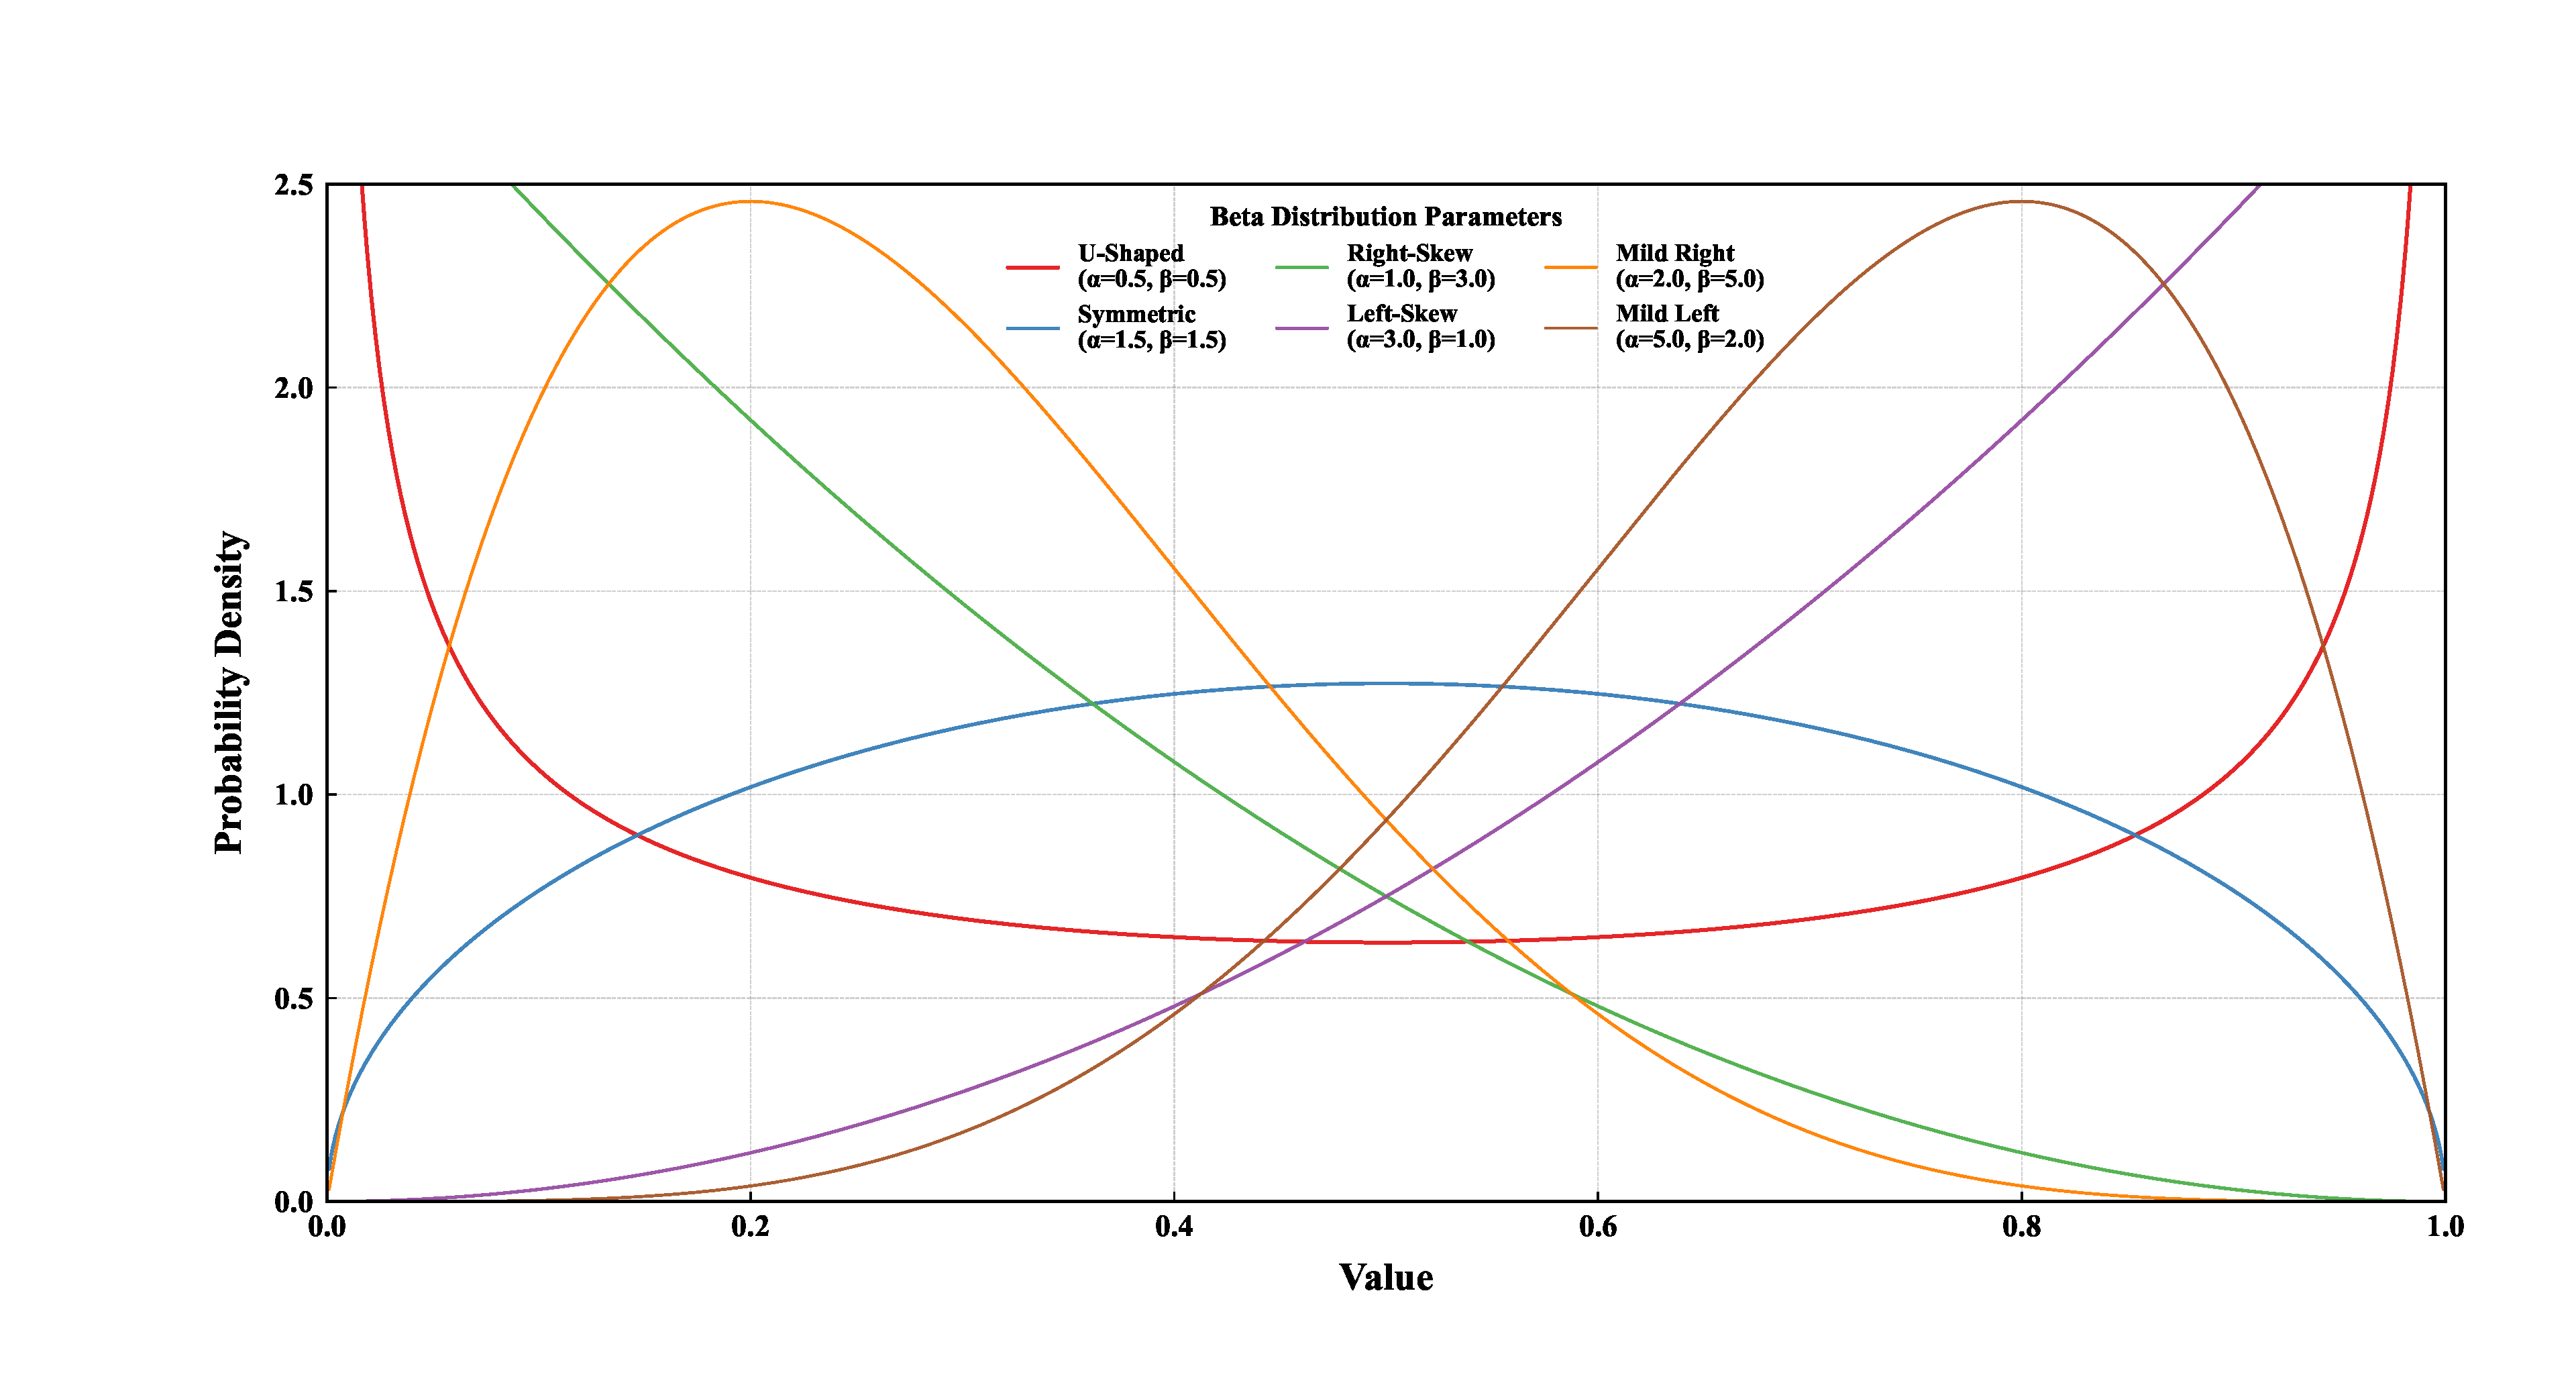
\includegraphics[width=0.8\textwidth]{figure1.pdf}}
\caption{Probability density function of Beta distribution.}
\label{figure:1}
\end{center}
\end{figure}



\section{Background}

\subsection{Beta Distribution}
\label{section:2.1}
The Beta distribution is a continuous probability distribution defined on the interval $[0,1]$, making it particularly well-suited for modeling probabilities. In this paper, we use it to represent the distribution of the expectation of a binary-valued reward. Its probability density function is given by
\begin{equation} 
\label{equation:1}
f(p; \alpha, \beta) = \frac{1}{\mathrm{B}(\alpha,\beta)} p^{\alpha - 1} (1 - p)^{\beta - 1}, \quad p \in [0,1] \text{ or } p \in (0,1), \quad \alpha > 0, \beta > 0,
\end{equation}
where $\mathrm{B}(\cdot,\cdot)$ denotes the Beta function, which serves as a normalization constant to ensure the probability density function integrates to one. Figure \ref{figure:1} illustrates the probability density function of the Beta distribution under various parameter settings.

The shape of the Beta distribution is primarily determined by the values of $\alpha$ and $\beta$, which control the concentration of probability mass and the skewness of the distribution. When $\alpha>1$ and $\beta>1$, the distribution is unimodal and bell-shaped, with the mode $\frac{\alpha-1}{\alpha+\beta-2}$ lying between 0 and 1. If $\alpha<1$ and $\beta<1$, the distribution becomes U-shaped, with higher densities near 0 and 1. When one of the parameters is less than 1 while the other is greater than 1, the distribution becomes highly skewed, concentrating mass near one endpoint. A special case occurs when $\alpha=\beta$, resulting in a symmetric distribution centered around $p=\frac{1}{2}$. This adaptability makes the Beta distribution a popular choice in probabilistic modeling contexts.

In terms of summary statistics, the mean of the Beta distribution is given by $\mathbb{E}[p]=\frac{\alpha}{\alpha+\beta}$, reflecting the balance between the two parameters. The variance is given by $\mathrm{Var}[p]=\frac{\alpha\beta}{(\alpha+\beta)^2(\alpha+\beta+1)}$, which decreases as the sum $\alpha+\beta$ increases, indicating greater certainty or concentration around the mean. 

\subsection{Policy Optimization}
Reinforcement learning provides an effective framework for training large language models by enabling them to learn policies through interaction with the environment and feedback signals. Among various reinforcement learning methods, policy gradient techniques are particularly prominent due to their ability to scale to high-dimensional action spaces typical in language generation tasks. Given a outcome reward function $R(q,o)$, the objective function in policy gradient methods is defined as:
\begin{align}
\label{equation:2}
    \mathcal{J}(\theta)&=\mathbb{E}_{q\sim\rho,\, o\sim\pi_\theta(\cdot| q)}\Bigl[R(q,o)\Bigr],
\end{align}
where $\rho$ represents the distribution of questions $q$, and $\pi_\theta(\cdot| q)$ denotes the parameterized policy model that defines the distribution over outputs $o$. According to the policy gradient theorem \citep{sutton1999policy}, the policy gradient for the objective in Eq.(\ref{equation:2}) is given by:
\begin{align}
\label{equation:3}
\nabla_\theta \mathcal{J}(\theta)= \mathbb{E}_{q\sim\rho,\, o\sim\pi_\theta(\cdot| q)}\Bigl[\nabla_\theta \log \pi_\theta(o| q)\, R(q,o)\Bigr].
\end{align}
In practice, directly using Eq.~(\ref{equation:3}) can lead to high variance in gradient estimates \citep{barto2021reinforcement}, which negatively impacts training stability. To mitigate this, policy gradient methods typically introduce an advantage function $A(q,o)$:
\begin{align}
\label{equation:4}
\nabla_\theta \mathcal{J}(\theta)&= \mathbb{E}_{q\sim\rho,\, o\sim\pi_\theta(\cdot| q)}\Bigl[\nabla_\theta \log \pi_\theta(o| q)\, A(q,o)\Bigr],
\end{align}
where $A(q,o)$ represents the relative advantage of a question-output pair $(q,o)$ compared to other pairs. The use of $A(q,o)$ primarily serves to reduce the variance in policy gradient estimation:
\begin{align}
\mathrm{Var}_{q\sim\rho,\, o\sim\pi_\theta(\cdot| q)}\Bigl[\nabla_\theta \log \pi_\theta(o| q)\, A(q,o)\Bigr].
\end{align}
The advantage function is commonly formulated as $A(q,o)=\frac{R(q,o)-\mu}{\sigma}$, where $\mu$ serves as a baseline for $R(q,o)$ to compare and $\sigma$ acts as a normalization term. With appropriate choices of $\mu$ and$\sigma$, the estimation of policy gradient remains unbiased while its variance is reduced.

REINFORCE with baseline \citep{team2025kimi,kool2019buy} defines $A(q,o)$ as
\begin{align}
\label{equation:5}
    A(q,o)=&R(q,o) - \mathbb{E}_{o'\sim\pi_\theta(\cdot| q)}\Bigl[ R(q,o') \Bigr]\notag\\
    \approx &R(q,o) - \mathrm{Mean}(\{R(q,o'_{j})\}_{j=1}^{m}),
\end{align}
where the baseline is the mean reward over a sampled group of outputs $\{(q, o'_j)\}_{j=1}^m$. This Monte Carlo estimate approximates the expected reward $\mathbb{E}_{o'\sim\pi_\theta(\cdot| q)}\Bigl[ R(q,o') \Bigr]$ and has been shown to effectively reduce the variance of policy gradient estimates \citep{wu2018variance}.

GRPO  \citep{guo2025deepseek,shao2024deepseekmath} defines $A(q,o)$ as:
\begin{align}
\label{equation:6}
    A(q,o)
     =&\frac{R(q,o)-\mathbb{E}_{o'\sim\pi_\theta(\cdot| q)}\Bigl[ R(q,o') \Bigr]}{\sqrt{\mathrm{Var}_{o'\sim\pi_\theta(\cdot| q)}[R(q,o')]}}\notag\\
    \approx &\frac{R(q,o) - \mathrm{Mean}(\{R(q,o'_{j})\}_{j=1}^{m})}{\sqrt{\mathrm{Var}(\{R(q,o'_{j})\}_{j=1}^{m})}},
\end{align}
Compared to REINFORCE with baseline, GRPO further uses the standard deviation of the rewards over the sampled set $\{(q, o'_j)\}_{j=1}^m$ to normalize the reward function. This normalization term can further reduce the variance in estimating policy gradient for high-variance reward functions.

PPO \citep{schulman2017proximal} further enhances stability by incorporating importance sampling and a clipping mechanism for off-policy updates:
\begin{align}
\label{equation:7}
    &\mathcal{J}(\theta)=\mathbb{E}_{q\sim \rho,o\sim \pi_{\theta_{\text{old}}}(o|q)}\Bigl[\min (\frac{\pi_{\theta}(o|q)}{\pi_{\theta_{\text{old}}(o|q)}}A(q,o),\text{clip}(\frac{\pi_{\theta}(o|q)}{\pi_{\theta_{\text{old}}}(o|q)},1-\varepsilon,1+\varepsilon)A(q,o))\Bigl],
\end{align}
where $\pi_{\theta_{old}}$ is the old policy and $\varepsilon$ is a hyperparameter that controls the range of clipping.


\section{Beta Normalization Policy Optimization}
In this section, we introduce our policy optimization method, BNPO, which employs a Beta distribution to normalize binary-valued reward functions. BNPO adapts to the evolving policy model during training by dynamically adjusting the parameters of the Beta distribution. We then provide a theoretical proof demonstrating that BNPO effectively reduces the variance of policy gradient estimates. Furthermore, we show that BNPO generalizes both REINFORCE with baseline and GRPO in the context of binary-valued rewards. Finally, we present an advantage decomposition mechanism to extend BNPO's applicability to more complex reward systems.
\paragraph{Beta Normalization}
We use the accuracy of an output $o$ with respect to a question $q$ as the reward function $R(q,o)$ as in DeepSeek-R1 \citep{guo2025deepseek}, i.e.,
\begin{align}
\label{equation:8}
    R(q,o)=
    \begin{cases}
    1, & \text{if } o \text{ contains the answer } a \text{ of the question }q,\\
    0, & \text{otherwise.}
    \end{cases}
\end{align}
Since the value of $R(q,o)$ is either 0 or 1, $R(q,o)$ can be treated as a random variable with Bernoulli distribution, i.e. 
\begin{align}
\label{equation:10}
&R(q,o)\sim \text{Bernoulli }(p(q)), \quad 0\leq p(q)\leq 1,\notag\\
&p(q)=\mathbb{E}_{o\sim\pi_\theta(\cdot| q)}[R(q, o) | q],
\end{align}
where $p(q)$ denotes the probability that output $o$ is correct for question $q$, and it is also the expected reward under the distribution $\pi_\theta(\cdot| q)$. As mentioned in Section \ref{section:2.1}, the Beta distribution is very suitable for modeling probability. Thus, we model $p(q)$ as a random variable with Beta distribution $f_{D}(p(q);a,b)$, where the parameters $a$ and $b$ control the shape of the distribution. These parameters can be estimated using Monte Carlo sampling.

As the policy model $\pi_\theta(\cdot| q)$ evolves during training, the distribution of $p(q)$ also changes dynamically. To account for these changes, we propose using an additional Beta distribution $f_{N}(p(q);\alpha,\beta)$ to normalize the reward function. The advantage function in our BNPO method is defined as:
\begin{align}
\label{equation:11}
    A_{\alpha, \beta}(q,o)= \frac{R(q,o)-p(q)}{f_{N}(p(q);\alpha,\beta)},
\end{align}
where $p(q)$ serves as the baseline, as in REINFORCE with baseline and GRPO, and $f_{N}(p(q);\alpha,\beta)$ is used to normalize the reward function $R(q,o)$.

\paragraph{The setting of $\alpha$ and $\beta$}
We dynamically adjust the parameters $(\alpha,\beta)$ in $f_{N}(p(q);\alpha,\beta)$ to ensure that $A_{\alpha, \beta}(q,o)$ adapts to the evolving distribution $f_{D}(p(q);a,b)$ during training. The primary goal in setting $\alpha$ and $\beta$ is to minimize the variance in policy gradient estimation. We present the following theorem to achieve it.
\begin{theorem}
\label{theorem:1}
Let \( q \sim \rho \) be a question and \( o \sim \pi_\theta(\cdot | q) \) be an output with reward \( R(q, o) \in \{0, 1\} \), where $R(q,o)$ follows a Bernoulli distribution with success probability \( p(q) = \mathbb{E}_{o\sim\pi_\theta(\cdot| q)}[R(q, o) | q] \), and that $p(q)$ follows a Beta distribution $f_{D}(p(q);a,b) $. Define the BNPO gradient estimator as
\[
g_{\alpha,\beta} = \nabla_\theta \log \pi(o | q) \frac{R(q,o)-p(q)}{f_{N}(p(q);\alpha,\beta)}.
\]
where $f_{N}(p(q);\alpha,\beta)$ is a Beta distribution. Under the assumption $\nabla_\theta \log \pi(o | q)$ is uncorrelated with $\frac{R(q,o)-p(q)}{f_{N}(p(q);\alpha,\beta)}$, the variance of the policy gradient estimator $\mathrm{Var}_{q\sim\rho,\, o\sim\pi_\theta(\cdot| q)}(g_{\alpha,\beta})$ is finite if and only if: \( \alpha < \frac{a + 3}{2} \) and \( \beta < \frac{b + 3}{2} \). Within this domain, $\mathrm{Var}_{q\sim\rho,\, o\sim\pi_\theta(\cdot| q)}(g_{\alpha,\beta})$ attains a unique minimum at:
\[
\alpha = 1 + \frac{a}{3}, \quad \beta = 1 + \frac{b}{3}.
\]
\end{theorem}
See Appendix \ref{appendix:1} for the proof. The above theorem demonstrates that the optimal parameter settings for minimizing the variance of the policy gradient are $\alpha = 1 + \frac{a}{3}$ and $\beta = 1 + \frac{b}{3}$. Thus, the choice of $(\alpha, \beta)$ depends on the values of $(a, b)$. We estimate $(a, b)$ using the method-of-moments approach and Monte Carlo sampling.

Given the following relationships:
\begin{align}
    \mathbb{E}[p(q)]&=\frac{a}{a+b},\notag\\
    \mathrm{Var}[p(q)]&=\frac{ab}{(a+b)^2(a+b+1)},
\end{align}
we can solve for $a$ and $b$ as:
\begin{align}
\label{equation:13}
&a = \Bigl(\frac{ \mathbb{E}[p(q)](1- \mathbb{E}[p(q)])}{\mathrm{Var}[p(q)]}-1\Bigr)\, \mathbb{E}[p(q)],\notag\\
&b = \Bigl(\frac{ \mathbb{E}[p(q)](1- \mathbb{E}[p(q)])}{\mathrm{Var}[p(q)]}-1\Bigr)\,(1- \mathbb{E}[p(q)]).
\end{align}
We then estimate $\mathbb{E}[p(q)]$ and $\mathrm{Var}[p(q)]$ using Monte Carlo methods to get $a$ and $b$:
\begin{align}
\label{equation:14}
    &\mathbb{E}[p(q)]\approx \text{Mean}(\{p(q_{i})\}_{i=1}^{n}),\quad \notag\\
&\mathrm{Var}[p(q)]\approx \text{Var}(\{p(q_{i})\}_{i=1}^{n}).
\end{align}

\paragraph{The interpretation of $\alpha$ and $\beta$}
The parameters $\alpha$ and $\beta$ can be understood in terms of the mean and variance of $f_{D}(p(q);a,b)$. The mean of $f_{D}(p(q);a,b)$ is given by $\frac{a}{a + b}$, representing the average reward of all $(q,o)$ pairs. The mode of $f_{N}(p(q);\alpha,\beta)$ is $\frac{\alpha - 1}{\alpha + \beta - 2} = \frac{a}{a + b}$, which corresponds to the value at which $f_{N}(p(q);\alpha,\beta)$ attains its maximum. This shows that the mean of $f_{D}(p(q);a,b)$ is equal to the mode of $f_{N}(p(q);\alpha,\beta)$. As a result, the reward function $R(q, o)$ is most normalized at the average reward $\frac{a}{a + b}$.

The variance of $f_{D}(p(q);a,b)$ decreases/increases as the sum $a+b$ increases/decreases. Since $\alpha + \beta = 2 + \frac{a + b}{3}$, the variance of $f_{N}(p(q);\alpha,\beta)$ behaves similarly: it decreases/increases as $a + b$ increases/decreases. Hence, $f_{N}(p(q);\alpha,\beta)$ adapts its parameters to align with the variance changes of $f_{D}(p(q);a,b)$.

\paragraph{REINFORCE and GRPO}
We now demonstrate that BNPO generalizes both REINFORCE with baseline and GRPO under binary-valued reward circumstances, reducing to each of these methods under specific settings for $\alpha$ and $\beta$.

REINFORCE with baseline defines the advantage function $A(q,o)$ as
\begin{align}
A(q,o)&= R(q,o)-\mathbb{E}_{o'\sim\pi_\theta(\cdot| q)}\Bigl[ R(q,o') \Bigr]\notag\\
&=R(q,o)-p(q)\notag\\
&=\frac{R(q,o)-p(q)}{f_{N}(p(q);1,1)}\notag\\
&=A_{1, 1}(q,o).
\end{align}
Therefore, BNPO reduces to REINFORCE if $f_{N}(p(q);\alpha,\beta)=f_{N}(p(q);1,1)$. Since RLOO \citep{kool2019buy,ahmadian2024back} is equivalent to REINFROCE with baseline up to a scaling constant \citep{liu2025understanding}, BNPO can also reduce to RLOO.

GRPO defines the advantage function $A(q,o)$ as
\begin{align}
    A(q,o)&= \frac{R(q,o)-\mathbb{E}_{o'\sim\pi_\theta(\cdot| q)}\Bigl[ R(q,o') \Bigr]}{\sqrt{\mathrm{Var}_{o'\sim\pi_\theta(\cdot| q)}[R(q,o')]}}\notag\\
    &=\frac{R(q,o)-p(q)}{\sqrt{p(q)(1-p(q))}}\notag\\
    &\propto \frac{R(q,o)-p(q)}{f_{N}(p(q);\frac{3}{2},\frac{3}{2})}\notag\\
    &=A_{\frac{3}{2},\frac{3}{2}}(q,o).
\end{align}
In training large language models, gradient clipping is commonly employed. Consequently, scaling the loss function by a constant does not affect the parameter update process. Consequently, BNPO reduces to GRPO if $f_{N}(p(q);\alpha,\beta)=f_{N}(p(q);\frac{3}{2},\frac{3}{2})$.

REINFORCE with a baseline and GRPO can be viewed as special cases of BNPO with fixed values of $(\alpha, \beta)$. In contrast, BNPO dynamically adjusts $(\alpha, \beta)$ during training to better align with the evolving policy model.

\paragraph{Advantage Decomposition}
To extend our method to more complex reward systems beyond a single binary reward function, we introduce an advantage decomposition mechanism. This approach enables the separate normalization of each individual reward component, leading to a more accurate estimation of the overall advantage function. Such decomposition is particularly beneficial in settings with multiple reward signals. For example, DeepSeek-R1 employs both format and accuracy rewards to ensure that model outputs not only follow the required structure but also produce correct answers.

Given $K$ binary-valued reward functions $\{R^{(1)}(q,o),R^{(2)}(q,o),\cdots, R^{(K)}(q,o)\}$, we decompose the overall advantage function $A(q,o)$ into $K$ sub-advantage functions $A^{(i)}(q,o)$ as follows:
\begin{align}
\label{equation:17}
    A(q,o)&=\frac{1}{K}\sum_{i=1}^{K}A^{(i)}(q,o)= \frac{1}{K}\sum_{i=1}^{K}\frac{R^{(i)}(q,o)-p(q)^{(i)}}{f_{N}(p(q)^{(i)};\alpha^{(i)},\beta^{(i)})}.
\end{align}
where each sub-advantage function $A^{(i)}(q,o)$ is computed for the corresponding reward function $R^{(i)}(q,o)$.

Unlike previous methods that first sum multiple reward functions and then compute the final advantage function, our approach calculates the advantage function for each individual reward function first, and then averages them to obtain the final advantage function. The key benefit of this approach is that it allows for separate normalization of each reward function, ensuring that the normalization of one function does not interfere with others.

We present the detailed implementation of our BNPO in Alg.(\ref{alg:1}). 

\begin{algorithm}[t]
    \caption{BNPO: Beta Normalization Policy Optimization}
    \label{alg:1}
    \begin{algorithmic}[1]
        \REQUIRE 
        Initial policy model $\pi_{\theta_{0}}$, $K$ binary-valued Reward model $R^{(i)}(q,o)$, training set $\mathcal{D}$,\\ number of steps $S$, number of PPO iterations $T$, batch size $n$, number of outputs $m$.
        \STATE Initialize policy model $\pi_\theta \gets \pi_{\theta_{0}}$.
        \FOR{$\text{step}=1$ \textbf{to} $S$}
            \STATE Update the old policy model $\pi_{\theta_{\text{old}}} \gets \pi_\theta$.
            \STATE Sample $n$ questions $q$ from $\mathcal{D}$.
            \STATE Sample $m$ outputs $o \sim \pi_{\theta_{\text{old}}}(\cdot | q)$ for each question $q$.
            \FOR{each question-output pair $(q,o)$}
            \FOR{$i=1$ \textbf{to} $K$}
                \STATE Compute the reward $R^{(i)}(q,o)$.
            \ENDFOR
            \ENDFOR
            \FOR{each question $q$}
            \STATE Estimate $p(q)$ in Eq.(\ref{equation:10}).
            \ENDFOR
            \STATE Estimate the parameters $a$ and $b$ in $f_{D}(p(q);a,b)$ by Eq.(\ref{equation:13}) and Eq.(\ref{equation:14}).
            \STATE Set the the parameters $\alpha$ and $\beta$  in $f_{N}(p(q);\alpha,\beta)$ as $\alpha=1+\frac{a}{3}$ and $\beta=1+\frac{b}{3}$.
            \FOR{each question-output pair $(q,o)$}
                \STATE Compute the advantage $A(q,o)$ by Eq.(\ref{equation:11}) and Eq.(\ref{equation:17}).
            \ENDFOR
            \FOR{$\text{iteration}=1$ \textbf{to} $T$}
                \STATE Update $\pi_\theta$ by maximizing Eq.(\ref{equation:7}).
            \ENDFOR
        \ENDFOR
        \ENSURE Optimized policy model $\pi_\theta$.
    \end{algorithmic}
\end{algorithm}




\section{Related Work}
Reinforcement learning has been widely adopted to align large language models with human preferences, as seen in systems like ChatGPT and DeepSeek-R1. ChatGPT \citep{ouyang2022training} employs PPO for policy optimization, which relies on a critic network to better estimate policy gradients. However, training a critic network is computationally intensive and memory-demanding, particularly for large language models. To address this, models such as DeepSeek-R1 and Qwen \citep{yang2024qwen2} adopt REINFORCE-based methods, which avoid the need for a critic network.

The original REINFORCE algorithm \citep{williams1992simple} estimates gradients through Monte Carlo sampling but often suffers from high variance, which can hinder learning stability and efficiency. To mitigate this issue, RLOO \citep{kool2019buy} introduces a baseline function that uses the mean reward of a group of samples as a reference, significantly reducing gradient variance, especially when batch sizes are small. ReMax \citep{li2024remax} builds on this idea by employing greedy decoding to obtain a baseline. GRPO \citep{shao2024deepseekmath} further refines this idea by normalizing each reward using the standard deviation of the group, reducing variance even more. REINFORCE++ \citep{hu2025reinforce++} goes a step further by leveraging the rewards of all samples to estimate the policy gradient, resulting in more stable and robust learning performance. However, these methods either lack proper normalization or rely on static normalization strategies, which are insufficient for adapting to the evolving nature of policy during training. In contrast, BNPO dynamically adjusts its normalization parameters in response to changes in the policy, effectively stabilizing training.


\section{Experiments}
In this section, we first describe the experimental setup in Section \ref{section:5.1}, followed by the presentation of results in Section \ref{section:5.2}. We then analyze training stability in Section \ref{section:5.3}. We finally show the evolution of the normalization of BNPO in Section \ref{section:5.4}.
\subsection{Experimental Settings}
\label{section:5.1}
\paragraph{Models}
To evaluate the effectiveness of BNPO, we conduct experiments on two publicly available base models of different scales: Qwen2.5-Math-1.5B and Qwen2.5-Math-7B \citep{yang2024qwen2, yang2024qwen2_math}.

\paragraph{Methods}
We compare BNPO method against several policy optimization methods, including REINFORCE, ReMax, GRPO, and REINFORCE++. Since RLOO is equivalent to REINFORCE with a baseline, we only report the results for REINFORCE with baseline.

\paragraph{Datasets}
For training, we utilize the full MATH dataset \citep{hendrycks2021measuring}, which consists of 7,500 diverse mathematical problems spanning a wide range of topics and difficulty levels.

For evaluation, we use four benchmark datasets: MATH500 \citep{hendrycks2021measuring,lightman2023let}, AMC23 \citep{aops_amc}, AIME2024 and AIME2025 \citep{aops_aime}. %These datasets represent varying levels of mathematical reasoning complexity and provide a rigorous framework for evaluating the model's generalization capabilities. By conducting evaluations on multiple datasets, we aim to offer a comprehensive analysis of model performance, both in-distribution and out-of-distribution.

\paragraph{Metrics}
We use pass@1 as the evaluation metric. For the AMC23, AIME 2024, and AIME 2025 datasets, we run the test set 16 times and report the average results, as these test sets are relatively small. We select the hyperparameters based on the best average performance.

\paragraph{Hyperparameters}
For all methods, we set the batch size 32, the number of outputs to 16, the number of PPO iterations to 1, the number of epochs to 5, and the learning rate to $10^{-6}$. The temperature is set to 1.0 during training and 0.6 during evaluation. We use the chat template of Qwen2.5-Math-7B and set the maximum question length to 1024 and the maximum output length to 3072, corresponding to the maximum context length of 4096 for Qwen-Math-1.5B and Qwen-Math-7B. We run all experiments on NVIDIA H20 GPUs.



\begin{table}[t]
    \centering
    \caption{The performance of different policy optimization methods on math datasets.}
    \label{table:1}
    \begin{tabular}{lcccccc}
        \toprule
        \textbf{Methods} & \textbf{MATH500} & \textbf{AMC23} & \textbf{AIME2024} & \textbf{AIME2025} & \textbf{Average}\\
        \midrule
        \multicolumn{6}{c}{\textit{Qwen2.5‑Math‑1.5B}} \\
        \midrule
        Base                                    & 28.0 & 27.3 & 6.0  & 3.1  &16.1 \\
        REINFORCE                               & 74.8 & 51.6 & 18.3  & 11.3  &39.0 \\
        ReMax                                   & 73.4 & \textbf{54.8} & 16.3  & 9.2  &38.4 \\
        GRPO                                    & \textbf{75.2} & 52.3 & \textbf{19.0}  & 9.4  &39.0 \\
        REINFORCE++                             & 72.8 & 54.1 & 16.9  & 9.4  &38.3\\
        BNPO                                    & 73.4 &54.5 & 18.3  & \textbf{11.5}  &\textbf{39.4} \\
        \midrule
        \multicolumn{6}{c}{\textit{Qwen2.5‑Math‑7B}}  \\
        \midrule
        Base                                    & 41.4 & 32.5 & 11.0  & 5.0   &22.5 \\
        REINFORCE                               & 78.4 & 61.7 & \textbf{34.2}  & 14.6   &47.2 \\
        ReMax                                   & 78.2 & 62.8 & 33.5 & \textbf{15.8}   &47.6 \\
        GRPO                                    & \textbf{78.6} & 64.5 & 32.3  & 12.9   &47.1 \\
        REINFORCE++                             & \textbf{78.6} & 64.4 & 32.1  & 12.3   &46.8 \\
        BNPO                                    & 77.0 & \textbf{68.8} & 32.1 & 13.3  &\textbf{47.8} \\
        \bottomrule
    \end{tabular}
\end{table}




\subsection{Results}
\label{section:5.2}
As shown in Table \ref{table:1}, BNPO achieves the highest average performance among all policy optimization methods for both the Qwen2.5-Math-1.5B and Qwen2.5-Math-7B base models, demonstrating its effectiveness and versatility. Notably, BNPO trained on Qwen2.5-Math-7B delivers significant improvements on the AMC23 dataset. In contrast, REINFORCE, GRPO, and REINFORCE++, which either lack normalization or rely on static normalization, exhibit suboptimal performance. Although ReMax achieves performance comparable to BNPO on the Qwen2.5-Math-7B model, it requires additional sampling to dynamically estimate the baseline, resulting in approximately 25\% longer training times in our experiments.




\subsection{Training Stability}
\label{section:5.3}
We have demonstrated in Theorem \ref{theorem:1} that BNPO effectively reduces gradient variance, thereby enhancing training stability. Given the substantial computational cost of training large language models, maintaining stable training dynamics is crucial. To evaluate this, we use the gradient norm, an indicator of policy variance, as a proxy for training stability.

As shown in Figure \ref{figure:2}, BNPO exhibits the highest stability among the methods, with consistently stable gradient norms throughout training. In contrast, GRPO, REINFORCE, and REINFORCE++ show significant fluctuations, indicating less stable training. These results highlight the benefit of BNPO’s dynamic normalization mechanism over the static normalization used in GRPO and REINFORCE++. While ReMax achieves good stability, it incurs greater computational overhead.


\subsection{Evolution of Normalization}
\label{section:5.4}
Our BNPO method dynamically adjusts the parameters \((\alpha, \beta)\) in the normalization \(f_{N}(p(q); \alpha, \beta)\) to ensure that the advantage function \(A_{\alpha, \beta}(q, o)\) remains aligned with the evolving expected reward distribution \(f_{D}(p(q); a, b)\) throughout training. We have further provided an interpretation of \(\alpha\) and \(\beta\) in terms of the mean and variance of \(f_{D}(p(q); a, b)\), demonstrating how they can be related to \(\mathbb{E}[p(q)]\) and \(\mathrm{Var}[p(q)]\).

To illustrate this relationship, Figure~\ref{figure:3} presents the evolution of \((\mathbb{E}[p(q)], \mathrm{Var}[p(q)], \alpha, \beta)\) over the course of training. As shown, the parameters \(\alpha\) and \(\beta\) effectively adapt in response to changes in the mean and variance of \(p(q)\), validating the adaptive capability of BNPO's normalization mechanism.

\begin{figure}[t]
\begin{center}
\centerline{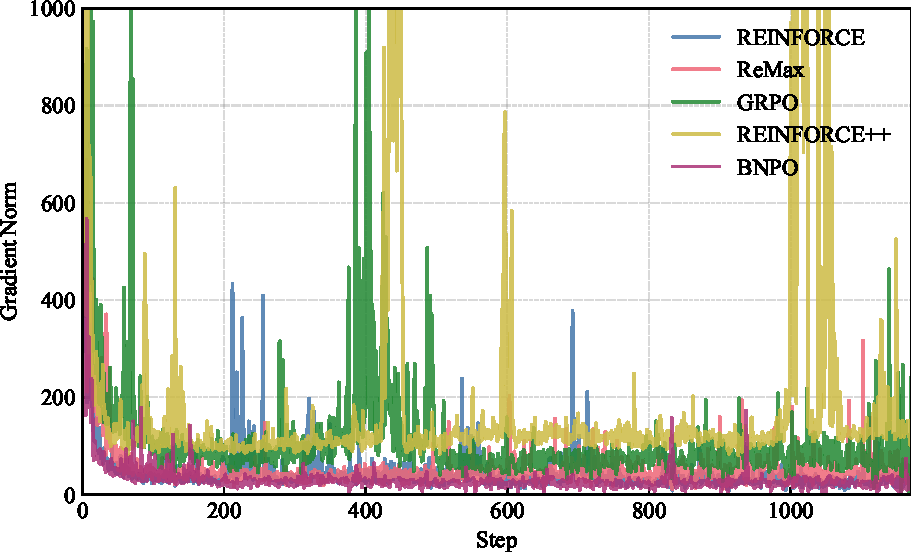
\includegraphics[width=0.6\textwidth]{figure2.pdf}}
\caption{The norm of gradient during training.}
\label{figure:2}
\end{center}
\end{figure}

\begin{figure}[h]
\begin{center}
\centerline{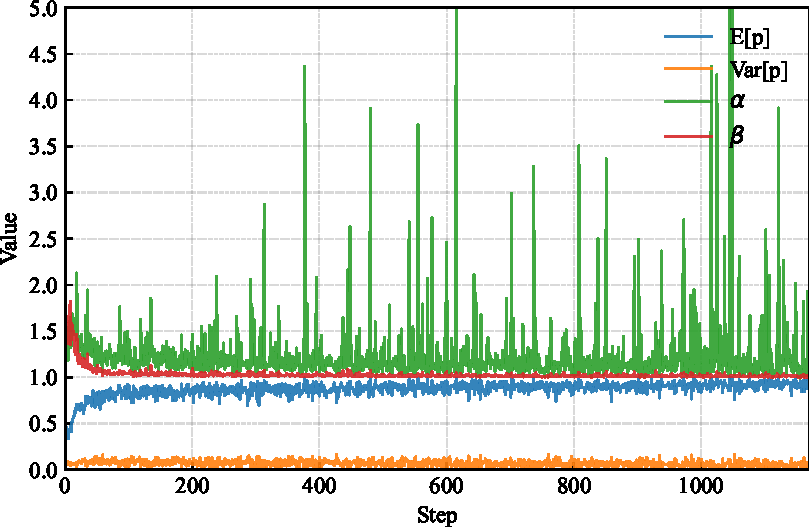
\includegraphics[width=0.6\textwidth]{figure3.pdf}}
\caption{The values of $(\mathbb{E}[p(q)],\mathrm{Var}[p(q)], \alpha,\beta)$ during training.}
\label{figure:3}
\end{center}
\end{figure}



\section{Limitations}
\paragraph{Multi-valued or Continuous Reward Functions}
Our BNPO is designed for binary-valued reward functions. To extend it to multi-valued rewards, one potential approach is to decompose the original reward into a set of binary-valued components. Another possibility is to employ the Dirichlet distribution as a normalization term, which naturally generalizes the Beta distribution to multi-valued settings. For continuous reward functions, the appropriate normalization method depends heavily on the specific form of the reward, making it challenging to develop a universal solution. Designing a general normalization method for continuous rewards remains a direction for future work.

\paragraph{Extension of Theorem \ref{theorem:1}}
Theorem \ref{theorem:1} is established under the assumption of binary-valued rewards, which limits its general applicability. However, as discussed in the interpretation of the parameters $\alpha$ and $\beta$, their values can be related to the mean and variance of $p(q)$. This suggests a promising direction: developing theoretical frameworks based on assumptions about the statistical properties (e.g., mean and variance) of $p(q)$, rather than restricting to binary rewards. Extending the theory in this way is a area of ongoing exploration.



\section{Conclusion}
In this paper, we propose a new policy optimization methods, BNPO, which use Beta distribution to normalize the reward function. We find that the expectation of a binary-valued reward function can be treated as a random variable with Beta distribution, thus, we use another Beta distribution as the normalize term. BNPO can adaptively adjust its parameters in normalization term to match with the evolution of distribution of the expected reward. We theoretically prove that BNPO can effectively reduce the variance in estimating policy gradient. We also that BNPO can reduces to REINFORCE with baseline and GRPO under binary-valued reward circumstance. In order to account for more complex reward systems, we further propose a advantage decomposition mechanism to make BNPO more applicable. Finally, we conduct extensive experiments to verify the effectiveness of our BNPO.






\bibliographystyle{plainnat}
\bibliography{cite.bib}


%%%%%%%%%%%%%%%%%%%%%%%%%%%%%%%%%%%%%%%%%%%%%%%%%%%%%%%%%%%%

\newpage


\appendix

\appendix
\setcounter{theorem}{0}


\section{Proof}
\label{appendix:1}

\begin{theorem}
Let \( q \sim \rho \) be a question and \( o \sim \pi_\theta(\cdot | q) \) be an output with reward \( R(q, o) \in \{0, 1\} \), where $R(q,o)$ follows a Bernoulli distribution with success probability \( p(q) = \mathbb{E}_{o\sim\pi_\theta(\cdot| q)}[R(q, o) | q] \), and that $p(q)$ follows a Beta distribution $f_{D}(p(q);a,b) $. Define the BNPO gradient estimator as
\[
g_{\alpha,\beta} = \nabla_\theta \log \pi(o | q) \frac{R(q,o)-p(q)}{f_{N}(p(q);\alpha,\beta)}.
\]
where $f_{N}(p(q);\alpha,\beta)$ is a Beta distribution. Under the assumption $\nabla_\theta \log \pi(o | q)$ is uncorrelated with $\frac{R(q,o)-p(q)}{f_{N}(p(q);\alpha,\beta)}$, the variance of the policy gradient estimator $\mathrm{Var}_{q\sim\rho,\, o\sim\pi_\theta(\cdot| q)}(g_{\alpha,\beta})$ is finite if and only if: \( \alpha < \frac{a + 3}{2} \) and \( \beta < \frac{b + 3}{2} \). Within this domain, $\mathrm{Var}_{q\sim\rho,\, o\sim\pi_\theta(\cdot| q)}(g_{\alpha,\beta})$ attains a unique minimum at:
\[
\alpha = 1 + \frac{a}{3}, \quad \beta = 1 + \frac{b}{3}.
\]
\end{theorem}

\begin{proof}
\subsection*{1. Variance Expression}
Expand the variance using its definition:
\begin{align*}
    \mathrm{Var}(g_{\alpha,\beta}) &= \mathbb{E}\left[\left(\nabla_\theta \log \pi(o \mid q) \cdot \frac{R(q,o)-p(q)}{f_N(p(q);\alpha,\beta)}\right)^2\right] \nonumber \\
    &\quad - \left(\mathbb{E}\left[\nabla_\theta \log \pi(o \mid q) \cdot \frac{R(q,o)-p(q)}{f_N(p(q);\alpha,\beta)}\right]\right)^2.
\end{align*}
Simplify the mean term using the assumption and $\mathbb{E}[\frac{R(q,o)-p(q)}{f_N(p(q);\alpha,\beta)}|q]=0$:
\begin{equation*}
    \mathbb{E}\left[\nabla_\theta \log \pi(o \mid q) \cdot \frac{R(q,o)-p(q)}{f_N(p(q);\alpha,\beta)}\right] = 0.
\end{equation*}
Therefore:
\begin{equation*}
    \mathrm{Var}(g_{\alpha,\beta}) = \mathbb{E}\left[\left(\nabla_\theta \log \pi(o \mid q)\right)^2 \cdot \frac{(R(q,o)-p(q))^2}{f_N(p(q);\alpha,\beta)^2}\right].
\end{equation*}

Under the assumption, the variance of the gradient estimator \( g_{\alpha,\beta} \) is proportional to:
\begin{equation*}
    \mathrm{Var}(g_{\alpha,\beta}) \propto \mathbb{E}_{q \sim \rho} \mathbb{E}_o \left[ \frac{(R(q,o)-p(q))^2}{f_{N}(p(q);\alpha,\beta)^2} \right].
\end{equation*}
For $R(q,o) \in \{0,1\}$, we have that
    \begin{equation*}
        \mathbb{E}_o \left[ (R - p(q))^2 | q \right] = p(q)(1 - p(q)).
    \end{equation*}
    Substituting the weight function:
    \begin{align*}
        \frac{p(q)(1 - p(q))}{f_{N}(p(q);\alpha,\beta)^2} &= \frac{p(q)(1 - p(q))}{\left(\frac{1}{B(\alpha,\beta)} p(q)^{\alpha-1}(1-p(q))^{\beta-1}\right)^2} \\
        &= B(\alpha,\beta)^2 \cdot p(q)^{3 - 2\alpha}(1-p(q))^{3 - 2\beta}.
    \end{align*}
Unper $p\sim f_{D}(p(q);a,b)$, the expectation integrates the above expression over the Beta-distributed $p$ becomes
\begin{equation*}
    \mathbb{E}_p \left[ p^{3 - 2\alpha}(1-p)^{3 - 2\beta} \right] = \frac{B(a + 3 - 2\alpha, b + 3 - 2\beta)}{B(a,b)},
\end{equation*}
Thus, we have that
\begin{equation*}
    \mathrm{Var}(g_{\alpha,\beta}) \propto B(\alpha,\beta)^2 \cdot \frac{B(a + 3 - 2\alpha, b + 3 - 2\beta)}{B(a,b)}.
\end{equation*}

\subsection*{2. Domain of Finiteness}
The Beta function \( B(x,y) \) converges iff \( x > 0 \) and \( y > 0 \). For convergence of \( B(a + 3 - 2\alpha, b + 3 - 2\beta) \):
\begin{align*}
    a + 3 - 2\alpha > 0 &\implies \alpha < \frac{a + 3}{2}, \\
    b + 3 - 2\beta > 0 &\implies \beta < \frac{b + 3}{2}.
\end{align*}

\subsection*{3. Boundary Behavior}
As \( \alpha \to \frac{a + 3}{2}^- \) or \( \beta \to \frac{b + 3}{2}^- \):
\begin{equation*}
    B(a + 3 - 2\alpha, b + 3 - 2\beta) \to \infty \implies \mathrm{Var}(g_{\alpha,\beta}) \to +\infty.
\end{equation*}

\subsection*{4. Optimal Parameters}
Define \( L(\alpha,\beta) = \ln \mathrm{Var}(g_{\alpha,\beta}) \):
\begin{equation*}
    L =  2\ln B(\alpha,\beta) + \ln B(a + 3 - 2\alpha, b + 3 - 2\beta) - \ln B(a,b).
\end{equation*}
The partial derivatives are:
\begin{equation*}
    \frac{\partial L}{\partial \alpha} = 2\left[\psi(\alpha) - \psi(\alpha + \beta)\right] - 2\left[\psi(a + 3 - 2\alpha) - \psi(a + b + 6 - 2\alpha - 2\beta)\right],
\end{equation*}
\begin{equation*}
    \frac{\partial L}{\partial \beta} = 2\left[\psi(\beta) - \psi(\alpha + \beta)\right] - 2\left[\psi(b + 3 - 2\beta) - \psi(a + b + 6 - 2\alpha - 2\beta)\right],
\end{equation*}
where \( \psi(x) = \frac{d}{dx}\ln \Gamma(x) \) and $\Gamma(x)$ is the gamma function. Setting \( \partial L/\partial \alpha = 0 \) and \( \partial L/\partial \beta = 0 \):
\begin{equation*}
    \psi(\alpha) - \psi(\alpha + \beta) = \psi(a + 3 - 2\alpha) - \psi(a + b + 6 - 2\alpha - 2\beta).
\end{equation*}
\begin{equation*}
    \psi(\beta) - \psi(\alpha + \beta) = \psi(b + 3 - 2\beta) - \psi(a + b + 6 - 2\alpha - 2\beta).
\end{equation*}
Substituting \( \alpha = 1 + \frac{a}{3} \) and \( \beta = 1 + \frac{b}{3} \) satisfies this identity through digamma function properties.

\subsection*{5. Strict Convexity}
We compute the Hessian matrix $H$ for $L(\alpha,\beta)$ at $(\alpha_0, \beta_0)$. 

Let $\psi_1(x) = \frac{d}{dx}\psi(x)$ be the trigamma function. Let $X_\alpha = \alpha_0 = 1+a/3$ and $X_\beta = \beta_0 = 1+b/3$. Let $S_{sum} = \alpha_0+\beta_0 = 2+(a+b)/3$.

The arguments for the other digamma terms at the solution become:
$a-2\alpha_0+3 = 1+a/3 = X_\alpha$.
$b-2\beta_0+3 = 1+b/3 = X_\beta$.
$a+b-2\alpha_0-2\beta_0+6 = (a+b)/3+2 = S_{sum}$.

The second partial derivatives are:
\begin{align*} \frac{\partial^2 L}{\partial \alpha^2} = 2\psi_1(\alpha) - 2\psi_1(\alpha+\beta) + 4\psi_1(a-2\alpha+3) - 4\psi_1(a+b-2\alpha-2\beta+6). \end{align*}
At $(\alpha_0,\beta_0)$:
$H_{11} = 2\psi_1(X_\alpha) - 2\psi_1(S_{sum}) + 4\psi_1(X_\alpha) - 4\psi_1(S_{sum}) = 6\psi_1(X_\alpha) - 6\psi_1(S_{sum})$.
By symmetry:
$H_{22} = 6\psi_1(X_\beta) - 6\psi_1(S_{sum})$.
The mixed partial derivative:
\begin{align*} \frac{\partial^2 L}{\partial \alpha \partial \beta} &= -2\psi_1(\alpha+\beta) - (-2)\psi_1(a+b-2\alpha-2\beta+6)(-2) \\ &= -2\psi_1(\alpha+\beta) - 4\psi_1(a+b-2\alpha-2\beta+6). \end{align*}
At $(\alpha_0,\beta_0)$:
$H_{12} = -2\psi_1(S_{sum}) - 4\psi_1(S_{sum}) = -6\psi_1(S_{sum})$.

For a minimum, $H$ must be positive definite.

1. $H_{11} > 0$:
$H_{11} = 6(\psi_1(X_\alpha) - \psi_1(S_{sum})) = 6(\psi_1(1+a/3) - \psi_1(2+(a+b)/3))$.
Since $a,b>0$, we have $X_\beta = 1+b/3 > 0$. Thus $X_\alpha = 1+a/3 < 1+a/3 + (1+b/3) = S_{sum}$.
The trigamma function $\psi_1(x)$ is strictly decreasing for $x>0$. Since $X_\alpha < S_{sum}$ (and $X_\alpha, S_{sum} >0$), $\psi_1(X_\alpha) > \psi_1(S_{sum})$. Thus $H_{11} > 0$. Similarly $H_{22} > 0$.

2. $\det(H) = H_{11}H_{22} - H_{12}^2 > 0$:
\begin{align*} &\det(H) \\
=& (6\psi_1(X_\alpha) - 6\psi_1(S_{sum}))(6\psi_1(X_\beta) - 6\psi_1(S_{sum})) - (-6\psi_1(S_{sum}))^2 \\ 
=& 36 [ \psi_1(X_\alpha)\psi_1(X_\beta) - \psi_1(X_\alpha)\psi_1(S_{sum}) - \psi_1(X_\beta)\psi_1(S_{sum}) + \psi_1(S_{sum})^2 - \psi_1(S_{sum})^2 ] \\ 
=& 36 [ \psi_1(X_\alpha)\psi_1(X_\beta) - \psi_1(S_{sum})(\psi_1(X_\alpha)+\psi_1(X_\beta)) ].\end{align*}
For $\det(H)>0$, we need $\psi_1(X_\alpha)\psi_1(X_\beta) - \psi_1(S_{sum})(\psi_1(X_\alpha)+\psi_1(X_\beta)) > 0$.
Since $\psi_1(x)>0$ for $x>0$, we can divide by $\psi_1(X_\alpha)\psi_1(X_\beta)\psi_1(S_{sum})$:
\[ \frac{1}{\psi_1(S_{sum})} - \left(\frac{1}{\psi_1(X_\beta)} + \frac{1}{\psi_1(X_\alpha)}\right) > 0 \implies \frac{1}{\psi_1(X_\alpha+X_\beta)} > \frac{1}{\psi_1(X_\alpha)} + \frac{1}{\psi_1(X_\beta)}. \]
Let $f(x) = 1/\psi_1(x)$. The inequality is $f(X_\alpha+X_\beta) > f(X_\alpha) + f(X_\beta)$.
The function $f(x)=1/\psi_1(x)$ is strictly convex on $(0, \infty)$.

As $x \to 0^+$, $\psi_1(x) \to \infty$, so $f(x) = 1/\psi_1(x) \to 0$. So we can define $f(0)=0$.
For a strictly convex function $f$ with $f(0)=0$:
For $x,y>0$, $f(x) = f(\frac{x}{x+y}(x+y) + \frac{y}{x+y} \cdot 0) < \frac{x}{x+y}f(x+y) + \frac{y}{x+y}f(0) = \frac{x}{x+y}f(x+y)$.
Similarly, $f(y) < \frac{y}{x+y}f(x+y)$.
Summing these gives $f(x)+f(y) < f(x+y)$.
The strict inequality holds because $X_\alpha = 1+a/3 > 0$ and $X_\beta = 1+b/3 > 0$.
Therefore, the Hessian matrix is positive definite at $(\alpha_0, \beta_0)$. Since the domain for $(\alpha,\beta)$ (where variance is finite, and $\alpha,\beta>0$) is a convex set, this implies that $(\alpha_0, \beta_0)$ is a unique minimum.
\end{proof}




\section{Experiments}
To evaluate the effectiveness of the advantage decomposition method, we incorporate an additional format reward following DeepSeek-R1. Since Qwen2.5-Math-1.5B and Qwen2.5-Math-7B exhibit limited instruction-following capabilities, making it difficult for them to learn from the format reward, we use Qwen2.5-1.5B-Instruct as the base model. We denote GRPO and REINFORCE++ with advantage decomposition as AD-GRPO and AD-REINFORCE++, respectively. Note that REINFORCE and ReMax do not include normalization and are therefore excluded from this comparison.

As shown in Table \ref{table:2}, both AD-GRPO and AD-REINFORCE++ achieve slight improvements over their original counterparts. BNPO continues to deliver the best average performance. However, since the format reward surpasses 90\% after only 100 training iterations, the overall performance gains from advantage decomposition are relatively modest.


\begin{table}[h]
    \centering
    \caption{The performance of policy optimization methods with and without advantage decomposition. }
    \label{table:2}
    \begin{tabular}{lcccccc}
        \toprule
        \textbf{Methods} & \textbf{MATH500} & \textbf{AMC23} & \textbf{AIME2024} & \textbf{AIME2025} & \textbf{Average}\\
        \midrule
        \multicolumn{6}{c}{\textit{Qwen2.5‑1.5B-Instruct}} \\
        \midrule
        Base                                    & 14.2 & 7.3 & 1.3  & 0.2  &5.8 \\
        GRPO                                    & 60.0 & 35.5 &  4.6  & 0.8  &25.2 \\
        REINFORCE++                             & 58.2 & 32.2 & \textbf{6.0}  & 1.9  &24.6 \\
        \midrule
        AD-GRPO                                 &  \textbf{61.6} & 34.1 & 3.8  &  \textbf{2.9}  &25.6 \\
        AD-REINFORCE++                          & 58.0 & 35.6 & 4.2  & 1.9  &24.9 \\
        AD-BNPO                                 & 61.4 & \textbf{36.3} & 3.8   & 1.9  & \textbf{25.8} \\
        \bottomrule
    \end{tabular}
\end{table}

\iffalse

%%%%%%%%%%%%%%%%%%%%%%%%%%%%%%%%%%%%%%%%%%%%%%%%%%%%%%%%%%%%

\newpage
\section*{NeurIPS Paper Checklist}

%%% BEGIN INSTRUCTIONS %%%
The checklist is designed to encourage best practices for responsible machine learning research, addressing issues of reproducibility, transparency, research ethics, and societal impact. Do not remove the checklist: {\bf The papers not including the checklist will be desk rejected.} The checklist should follow the references and follow the (optional) supplemental material.  The checklist does NOT count towards the page
limit. 

Please read the checklist guidelines carefully for information on how to answer these questions. For each question in the checklist:
\begin{itemize}
    \item You should answer \answerYes{}, \answerNo{}, or \answerNA{}.
    \item \answerNA{} means either that the question is Not Applicable for that particular paper or the relevant information is Not Available.
    \item Please provide a short (1–2 sentence) justification right after your answer (even for NA). 
   % \item {\bf The papers not including the checklist will be desk rejected.}
\end{itemize}

{\bf The checklist answers are an integral part of your paper submission.} They are visible to the reviewers, area chairs, senior area chairs, and ethics reviewers. You will be asked to also include it (after eventual revisions) with the final version of your paper, and its final version will be published with the paper.

The reviewers of your paper will be asked to use the checklist as one of the factors in their evaluation. While "\answerYes{}" is generally preferable to "\answerNo{}", it is perfectly acceptable to answer "\answerNo{}" provided a proper justification is given (e.g., "error bars are not reported because it would be too computationally expensive" or "we were unable to find the license for the dataset we used"). In general, answering "\answerNo{}" or "\answerNA{}" is not grounds for rejection. While the questions are phrased in a binary way, we acknowledge that the true answer is often more nuanced, so please just use your best judgment and write a justification to elaborate. All supporting evidence can appear either in the main paper or the supplemental material, provided in appendix. If you answer \answerYes{} to a question, in the justification please point to the section(s) where related material for the question can be found.

IMPORTANT, please:
\begin{itemize}
    \item {\bf Delete this instruction block, but keep the section heading ``NeurIPS Paper Checklist"},
    \item  {\bf Keep the checklist subsection headings, questions/answers and guidelines below.}
    \item {\bf Do not modify the questions and only use the provided macros for your answers}.
\end{itemize} 
 

%%% END INSTRUCTIONS %%%


\begin{enumerate}

\item {\bf Claims}
    \item[] Question: Do the main claims made in the abstract and introduction accurately reflect the paper's contributions and scope?
    \item[] Answer: \answerYes{} % Replace by \answerYes{}, \answerNo{}, or \answerNA{}.
    \item[] Justification: See the abstract and introduction.
    \item[] Guidelines:
    \begin{itemize}
        \item The answer NA means that the abstract and introduction do not include the claims made in the paper.
        \item The abstract and/or introduction should clearly state the claims made, including the contributions made in the paper and important assumptions and limitations. A No or NA answer to this question will not be perceived well by the reviewers. 
        \item The claims made should match theoretical and experimental results, and reflect how much the results can be expected to generalize to other settings. 
        \item It is fine to include aspirational goals as motivation as long as it is clear that these goals are not attained by the paper. 
    \end{itemize}

\item {\bf Limitations}
    \item[] Question: Does the paper discuss the limitations of the work performed by the authors?
    \item[] Answer: \answerYes{} % Replace by \answerYes{}, \answerNo{}, or \answerNA{}.
    \item[] Justification: See Section 6.
    \item[] Guidelines:
    \begin{itemize}
        \item The answer NA means that the paper has no limitation while the answer No means that the paper has limitations, but those are not discussed in the paper. 
        \item The authors are encouraged to create a separate "Limitations" section in their paper.
        \item The paper should point out any strong assumptions and how robust the results are to violations of these assumptions (e.g., independence assumptions, noiseless settings, model well-specification, asymptotic approximations only holding locally). The authors should reflect on how these assumptions might be violated in practice and what the implications would be.
        \item The authors should reflect on the scope of the claims made, e.g., if the approach was only tested on a few datasets or with a few runs. In general, empirical results often depend on implicit assumptions, which should be articulated.
        \item The authors should reflect on the factors that influence the performance of the approach. For example, a facial recognition algorithm may perform poorly when image resolution is low or images are taken in low lighting. Or a speech-to-text system might not be used reliably to provide closed captions for online lectures because it fails to handle technical jargon.
        \item The authors should discuss the computational efficiency of the proposed algorithms and how they scale with dataset size.
        \item If applicable, the authors should discuss possible limitations of their approach to address problems of privacy and fairness.
        \item While the authors might fear that complete honesty about limitations might be used by reviewers as grounds for rejection, a worse outcome might be that reviewers discover limitations that aren't acknowledged in the paper. The authors should use their best judgment and recognize that individual actions in favor of transparency play an important role in developing norms that preserve the integrity of the community. Reviewers will be specifically instructed to not penalize honesty concerning limitations.
    \end{itemize}

\item {\bf Theory assumptions and proofs}
    \item[] Question: For each theoretical result, does the paper provide the full set of assumptions and a complete (and correct) proof?
    \item[] Answer: \answerYes{} % Replace by \answerYes{}, \answerNo{}, or \answerNA{}.
    \item[] Justification: See Appendix A.
    \item[] Guidelines:
    \begin{itemize}
        \item The answer NA means that the paper does not include theoretical results. 
        \item All the theorems, formulas, and proofs in the paper should be numbered and cross-referenced.
        \item All assumptions should be clearly stated or referenced in the statement of any theorems.
        \item The proofs can either appear in the main paper or the supplemental material, but if they appear in the supplemental material, the authors are encouraged to provide a short proof sketch to provide intuition. 
        \item Inversely, any informal proof provided in the core of the paper should be complemented by formal proofs provided in appendix or supplemental material.
        \item Theorems and Lemmas that the proof relies upon should be properly referenced. 
    \end{itemize}

    \item {\bf Experimental result reproducibility}
    \item[] Question: Does the paper fully disclose all the information needed to reproduce the main experimental results of the paper to the extent that it affects the main claims and/or conclusions of the paper (regardless of whether the code and data are provided or not)?
    \item[] Answer: \answerYes{} % Replace by \answerYes{}, \answerNo{}, or \answerNA{}.
    \item[] Justification: See Section 5.1.
    \item[] Guidelines:
    \begin{itemize}
        \item The answer NA means that the paper does not include experiments.
        \item If the paper includes experiments, a No answer to this question will not be perceived well by the reviewers: Making the paper reproducible is important, regardless of whether the code and data are provided or not.
        \item If the contribution is a dataset and/or model, the authors should describe the steps taken to make their results reproducible or verifiable. 
        \item Depending on the contribution, reproducibility can be accomplished in various ways. For example, if the contribution is a novel architecture, describing the architecture fully might suffice, or if the contribution is a specific model and empirical evaluation, it may be necessary to either make it possible for others to replicate the model with the same dataset, or provide access to the model. In general. releasing code and data is often one good way to accomplish this, but reproducibility can also be provided via detailed instructions for how to replicate the results, access to a hosted model (e.g., in the case of a large language model), releasing of a model checkpoint, or other means that are appropriate to the research performed.
        \item While NeurIPS does not require releasing code, the conference does require all submissions to provide some reasonable avenue for reproducibility, which may depend on the nature of the contribution. For example
        \begin{enumerate}
            \item If the contribution is primarily a new algorithm, the paper should make it clear how to reproduce that algorithm.
            \item If the contribution is primarily a new model architecture, the paper should describe the architecture clearly and fully.
            \item If the contribution is a new model (e.g., a large language model), then there should either be a way to access this model for reproducing the results or a way to reproduce the model (e.g., with an open-source dataset or instructions for how to construct the dataset).
            \item We recognize that reproducibility may be tricky in some cases, in which case authors are welcome to describe the particular way they provide for reproducibility. In the case of closed-source models, it may be that access to the model is limited in some way (e.g., to registered users), but it should be possible for other researchers to have some path to reproducing or verifying the results.
        \end{enumerate}
    \end{itemize}


\item {\bf Open access to data and code}
    \item[] Question: Does the paper provide open access to the data and code, with sufficient instructions to faithfully reproduce the main experimental results, as described in supplemental material?
    \item[] Answer: \answerYes{} % Replace by \answerYes{}, \answerNo{}, or \answerNA{}.
    \item[] Justification: See the supplemental material.
    \item[] Guidelines:
    \begin{itemize}
        \item The answer NA means that paper does not include experiments requiring code.
        \item Please see the NeurIPS code and data submission guidelines (\url{https://nips.cc/public/guides/CodeSubmissionPolicy}) for more details.
        \item While we encourage the release of code and data, we understand that this might not be possible, so “No” is an acceptable answer. Papers cannot be rejected simply for not including code, unless this is central to the contribution (e.g., for a new open-source benchmark).
        \item The instructions should contain the exact command and environment needed to run to reproduce the results. See the NeurIPS code and data submission guidelines (\url{https://nips.cc/public/guides/CodeSubmissionPolicy}) for more details.
        \item The authors should provide instructions on data access and preparation, including how to access the raw data, preprocessed data, intermediate data, and generated data, etc.
        \item The authors should provide scripts to reproduce all experimental results for the new proposed method and baselines. If only a subset of experiments are reproducible, they should state which ones are omitted from the script and why.
        \item At submission time, to preserve anonymity, the authors should release anonymized versions (if applicable).
        \item Providing as much information as possible in supplemental material (appended to the paper) is recommended, but including URLs to data and code is permitted.
    \end{itemize}


\item {\bf Experimental setting/details}
    \item[] Question: Does the paper specify all the training and test details (e.g., data splits, hyperparameters, how they were chosen, type of optimizer, etc.) necessary to understand the results?
    \item[] Answer: \answerYes{} % Replace by \answerYes{}, \answerNo{}, or \answerNA{}.
    \item[] Justification: See Section 5.1.
    \item[] Guidelines:
    \begin{itemize}
        \item The answer NA means that the paper does not include experiments.
        \item The experimental setting should be presented in the core of the paper to a level of detail that is necessary to appreciate the results and make sense of them.
        \item The full details can be provided either with the code, in appendix, or as supplemental material.
    \end{itemize}

\item {\bf Experiment statistical significance}
    \item[] Question: Does the paper report error bars suitably and correctly defined or other appropriate information about the statistical significance of the experiments?
    \item[] Answer: \answerYes{} % Replace by \answerYes{}, \answerNo{}, or \answerNA{}.
    \item[] Justification: See Section 5.1 paragraph Metrics
    \item[] Guidelines:
    \begin{itemize}
        \item The answer NA means that the paper does not include experiments.
        \item The authors should answer "Yes" if the results are accompanied by error bars, confidence intervals, or statistical significance tests, at least for the experiments that support the main claims of the paper.
        \item The factors of variability that the error bars are capturing should be clearly stated (for example, train/test split, initialization, random drawing of some parameter, or overall run with given experimental conditions).
        \item The method for calculating the error bars should be explained (closed form formula, call to a library function, bootstrap, etc.)
        \item The assumptions made should be given (e.g., Normally distributed errors).
        \item It should be clear whether the error bar is the standard deviation or the standard error of the mean.
        \item It is OK to report 1-sigma error bars, but one should state it. The authors should preferably report a 2-sigma error bar than state that they have a 96\% CI, if the hypothesis of Normality of errors is not verified.
        \item For asymmetric distributions, the authors should be careful not to show in tables or figures symmetric error bars that would yield results that are out of range (e.g. negative error rates).
        \item If error bars are reported in tables or plots, The authors should explain in the text how they were calculated and reference the corresponding figures or tables in the text.
    \end{itemize}

\item {\bf Experiments compute resources}
    \item[] Question: For each experiment, does the paper provide sufficient information on the computer resources (type of compute workers, memory, time of execution) needed to reproduce the experiments?
    \item[] Answer: \answerYes{} % Replace by \answerYes{}, \answerNo{}, or \answerNA{}.
    \item[] Justification: See Section 5.1 
    \item[] Guidelines:
    \begin{itemize}
        \item The answer NA means that the paper does not include experiments.
        \item The paper should indicate the type of compute workers CPU or GPU, internal cluster, or cloud provider, including relevant memory and storage.
        \item The paper should provide the amount of compute required for each of the individual experimental runs as well as estimate the total compute. 
        \item The paper should disclose whether the full research project required more compute than the experiments reported in the paper (e.g., preliminary or failed experiments that didn't make it into the paper). 
    \end{itemize}
    
\item {\bf Code of ethics}
    \item[] Question: Does the research conducted in the paper conform, in every respect, with the NeurIPS Code of Ethics \url{https://neurips.cc/public/EthicsGuidelines}?
    \item[] Answer: \answerYes{} % Replace by \answerYes{}, \answerNo{}, or \answerNA{}.
    \item[] Justification: Our research conform, in every respect, with the NeurIPS Code of Ethics.
    \item[] Guidelines:
    \begin{itemize}
        \item The answer NA means that the authors have not reviewed the NeurIPS Code of Ethics.
        \item If the authors answer No, they should explain the special circumstances that require a deviation from the Code of Ethics.
        \item The authors should make sure to preserve anonymity (e.g., if there is a special consideration due to laws or regulations in their jurisdiction).
    \end{itemize}


\item {\bf Broader impacts}
    \item[] Question: Does the paper discuss both potential positive societal impacts and negative societal impacts of the work performed?
    \item[] Answer: \answerNA{} % Replace by \answerYes{}, \answerNo{}, or \answerNA{}.
    \item[] Justification: There is no societal impact of the work performed.
    \item[] Guidelines:
    \begin{itemize}
        \item The answer NA means that there is no societal impact of the work performed.
        \item If the authors answer NA or No, they should explain why their work has no societal impact or why the paper does not address societal impact.
        \item Examples of negative societal impacts include potential malicious or unintended uses (e.g., disinformation, generating fake profiles, surveillance), fairness considerations (e.g., deployment of technologies that could make decisions that unfairly impact specific groups), privacy considerations, and security considerations.
        \item The conference expects that many papers will be foundational research and not tied to particular applications, let alone deployments. However, if there is a direct path to any negative applications, the authors should point it out. For example, it is legitimate to point out that an improvement in the quality of generative models could be used to generate deepfakes for disinformation. On the other hand, it is not needed to point out that a generic algorithm for optimizing neural networks could enable people to train models that generate Deepfakes faster.
        \item The authors should consider possible harms that could arise when the technology is being used as intended and functioning correctly, harms that could arise when the technology is being used as intended but gives incorrect results, and harms following from (intentional or unintentional) misuse of the technology.
        \item If there are negative societal impacts, the authors could also discuss possible mitigation strategies (e.g., gated release of models, providing defenses in addition to attacks, mechanisms for monitoring misuse, mechanisms to monitor how a system learns from feedback over time, improving the efficiency and accessibility of ML).
    \end{itemize}
    
\item {\bf Safeguards}
    \item[] Question: Does the paper describe safeguards that have been put in place for responsible release of data or models that have a high risk for misuse (e.g., pretrained language models, image generators, or scraped datasets)?
    \item[] Answer: \answerNA{} % Replace by \answerYes{}, \answerNo{}, or \answerNA{}.
    \item[] Justification: Our paper poses no such risks
    \item[] Guidelines:
    \begin{itemize}
        \item The answer NA means that the paper poses no such risks.
        \item Released models that have a high risk for misuse or dual-use should be released with necessary safeguards to allow for controlled use of the model, for example by requiring that users adhere to usage guidelines or restrictions to access the model or implementing safety filters. 
        \item Datasets that have been scraped from the Internet could pose safety risks. The authors should describe how they avoided releasing unsafe images.
        \item We recognize that providing effective safeguards is challenging, and many papers do not require this, but we encourage authors to take this into account and make a best faith effort.
    \end{itemize}

\item {\bf Licenses for existing assets}
    \item[] Question: Are the creators or original owners of assets (e.g., code, data, models), used in the paper, properly credited and are the license and terms of use explicitly mentioned and properly respected?
    \item[] Answer: \answerYes{} % Replace by \answerYes{}, \answerNo{}, or \answerNA{}.
    \item[] Justification: We have cited the original paper that produced the code package or dataset.
    \item[] Guidelines:
    \begin{itemize}
        \item The answer NA means that the paper does not use existing assets.
        \item The authors should cite the original paper that produced the code package or dataset.
        \item The authors should state which version of the asset is used and, if possible, include a URL.
        \item The name of the license (e.g., CC-BY 4.0) should be included for each asset.
        \item For scraped data from a particular source (e.g., website), the copyright and terms of service of that source should be provided.
        \item If assets are released, the license, copyright information, and terms of use in the package should be provided. For popular datasets, \url{paperswithcode.com/datasets} has curated licenses for some datasets. Their licensing guide can help determine the license of a dataset.
        \item For existing datasets that are re-packaged, both the original license and the license of the derived asset (if it has changed) should be provided.
        \item If this information is not available online, the authors are encouraged to reach out to the asset's creators.
    \end{itemize}

\item {\bf New assets}
    \item[] Question: Are new assets introduced in the paper well documented and is the documentation provided alongside the assets?
    \item[] Answer: \answerNA{} % Replace by \answerYes{}, \answerNo{}, or \answerNA{}.
    \item[] Justification: Our paper does not release new assets.
    \item[] Guidelines:
    \begin{itemize}
        \item The answer NA means that the paper does not release new assets.
        \item Researchers should communicate the details of the dataset/code/model as part of their submissions via structured templates. This includes details about training, license, limitations, etc. 
        \item The paper should discuss whether and how consent was obtained from people whose asset is used.
        \item At submission time, remember to anonymize your assets (if applicable). You can either create an anonymized URL or include an anonymized zip file.
    \end{itemize}

\item {\bf Crowdsourcing and research with human subjects}
    \item[] Question: For crowdsourcing experiments and research with human subjects, does the paper include the full text of instructions given to participants and screenshots, if applicable, as well as details about compensation (if any)? 
    \item[] Answer: \answerNA{} % Replace by \answerYes{}, \answerNo{}, or \answerNA{}.
    \item[] Justification: Our paper does not involve crowdsourcing nor research with human subjects.
    \item[] Guidelines:
    \begin{itemize}
        \item The answer NA means that the paper does not involve crowdsourcing nor research with human subjects.
        \item Including this information in the supplemental material is fine, but if the main contribution of the paper involves human subjects, then as much detail as possible should be included in the main paper. 
        \item According to the NeurIPS Code of Ethics, workers involved in data collection, curation, or other labor should be paid at least the minimum wage in the country of the data collector. 
    \end{itemize}

\item {\bf Institutional review board (IRB) approvals or equivalent for research with human subjects}
    \item[] Question: Does the paper describe potential risks incurred by study participants, whether such risks were disclosed to the subjects, and whether Institutional Review Board (IRB) approvals (or an equivalent approval/review based on the requirements of your country or institution) were obtained?
    \item[] Answer: \answerNA{} % Replace by \answerYes{}, \answerNo{}, or \answerNA{}.
    \item[] Justification: Our paper does not involve crowdsourcing nor research with human subjects.
    \item[] Guidelines:
    \begin{itemize}
        \item The answer NA means that the paper does not involve crowdsourcing nor research with human subjects.
        \item Depending on the country in which research is conducted, IRB approval (or equivalent) may be required for any human subjects research. If you obtained IRB approval, you should clearly state this in the paper. 
        \item We recognize that the procedures for this may vary significantly between institutions and locations, and we expect authors to adhere to the NeurIPS Code of Ethics and the guidelines for their institution. 
        \item For initial submissions, do not include any information that would break anonymity (if applicable), such as the institution conducting the review.
    \end{itemize}

\item {\bf Declaration of LLM usage}
    \item[] Question: Does the paper describe the usage of LLMs if it is an important, original, or non-standard component of the core methods in this research? Note that if the LLM is used only for writing, editing, or formatting purposes and does not impact the core methodology, scientific rigorousness, or originality of the research, declaration is not required.
    %this research? 
    \item[] Answer: \answerNA{} % Replace by \answerYes{}, \answerNo{}, or \answerNA{}.
    \item[] Justification: The core method of our paper does not involve LLMs as any important, original, or non-standard components.
    \item[] Guidelines:
    \begin{itemize}
        \item The answer NA means that the core method development in this research does not involve LLMs as any important, original, or non-standard components.
        \item Please refer to our LLM policy (\url{https://neurips.cc/Conferences/2025/LLM}) for what should or should not be described.
    \end{itemize}

\end{enumerate}
\fi

\end{document}